\documentclass[aspectratio=1610,dvipsnames,xcolor=table]{beamer}

\setbeamersize{text margin left=3mm,text margin right=3mm} 
\usepackage{t1enc}
\usepackage[magyar]{babel}
\usepackage{subcaption}
\usepackage[export]{adjustbox}
\usepackage[table]{xcolor}



\definecolor{szin1}{rgb}{0.5, 0.188, 0.478}
\definecolor{szin2}{RGB}{196, 203, 133}
\definecolor{szin3}{cmyk}{0, 0.7771, 0.5437, 0.8656}
\definecolor{szin4}{gray}{0.5}

\usepackage{graphics}
\usepackage{wrapfig}

\usetheme{Malmoe}
\usecolortheme{crane}



\begin{document}

\title{Féléves beadandó}
\author{Nagy Róbert és Bartók-Balogh Gábor}
\date{\today}
\subtitle{Prezentáció  \LaTeX-kel az \textbf{xcolor} csomagról}
\institute{Miskolci Egyetem}

 % titleslide
\frame[plain]{\maketitle}

    
    % slide 1 
\begin{frame}[fragile]{Az xcolor csomag alapjai}
    \begin{minipage}{0.6\textwidth}
        \begin{itemize}
           \item \onslide<1->\verb!\usepackage[<Opciók>]{xcolor}!
           \item \onslide<2->Az xcolor lehetővé teszi, hogy kiszínezzünk 					                              szöveget,táblázatot, rajzolt ábrákat, stb... 
           \item \onslide<3->Használhatunk névvel ellátott színeket
           \item \onslide<4->Alapból 19 darab van.
           \item \onslide<5->dvipsnames opcióval 68 darab
           \item \onslide<5->svgnames opcióval 151 darab 
           \item \onslide<5->x11names opcióval pedig 317 darab
        \end{itemize}
     \end{minipage} \hfill
\begin{minipage}{0.35\textwidth}    
            \begin{figure}
                \onslide<4->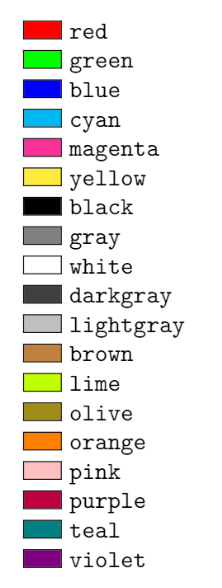
\includegraphics[scale=0.4]{img/szinek.png}
                \onslide<4->\caption{Névvel ellátott színek}
            \end{figure}
        \end{minipage}
    \end{frame}

    % slide 2
    \begin{frame}[fragile]{Az xcolor csomag alapjai}
        \begin{minipage}{0.8\textwidth}
            \begin{itemize}
                \item \onslide<1->Definiálhatunk saját színeket is.
                \item \onslide<2->\verb!\definecolor{<név>}{<Mód>}{<Értékek>}!
                \item \onslide<3->A mód lehet
                \begin{enumerate}
                    \item \onslide<4->rgb
                    \item \onslide<4->RGB
                    \item \onslide<4->cmyk
                    \item \onslide<4->gray    
                \end{enumerate}
                Például:
                \item \onslide<5->\verb!\definecolor{szin1}{rgb}{0.500, 0.188, 0.478}! 						\hfill \textcolor{szin1}{Szín1}
                \item \onslide<5->\verb!\definecolor{szin2}{RGB}{196, 203, 133}! \hfill 					\textcolor{szin2}{Szín2}
                \item \onslide<5->\verb!\definecolor{szin3}{cmyk}{0, 0.7771, 0.5437, 0.8656}! \hfill \textcolor{szin3}{Szín3}
                \item \onslide<5->\verb!\definecolor{szin4}{gray}{0.5}! \hfill 								\textcolor{szin4}{Szín4}
            \end{itemize}
                                                        
        \end{minipage} 
        
    \end{frame}
    
  
\begin{frame}[fragile]{Használat}
	
 	\onslide<1->\begin{block}{Megjegyzés}
 		Az esetben ha már betöltöttük az \textbf{xcolor} csomagot akkor a 'dvipsnames' 				szócskát a documentclassban megadva a package implementálása nélkül is gond 				nélkül tudjuk használni a csomagban elérhető színeket
	\end{block} 	
	
	\onslide<2->\begin{exampleblock}{Példa}
    {
       \verb!\documentclass[aspectratio=1610,dvipsnames]{beamer}!
    }
    \end{exampleblock}
	
	
\end{frame}

\begin{frame}[fragile]{Használat}
\begin{center}
Ha minden rendben betöltődött akkor pedig a következő példa képeken és kód részleteken láthatjuk,hogy hogyan néz ki az \textbf{xcolor package használata}
\noindent
{\color{Dandelion} \rule{\linewidth}{1mm}}
\end{center}
	
	\begin{figure}[H]
			 \onslide<2->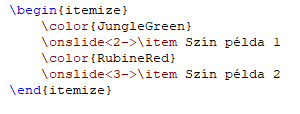
\includegraphics[scale=0.8]{img/itemszinezes.png}
			 \onslide<2->\caption{Itemek színezése}
	\end{figure}
\end{frame}


\begin{frame}[fragile]{Használat}

\begin{figure}[H]
\onslide<1->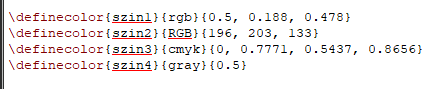
\includegraphics[scale=0.9]{img/itemszinezes2.1.png} 
\onslide<1->\caption{Saját szín definiálás}
\onslide<2->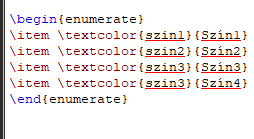
\includegraphics[scale=0.9]{img/itemszinezes2.png}
\onslide<2->\caption{Saját szín használata}
\end{figure}
\end{frame}

\begin{frame}[fragile]{Táblázat színezés}
\begin{center}

A \verb!\usepackage[table]{xcolor}! package implementálása után tudunk táblázatban is hasonló dolgokat alkotni.
\noindent
{\color{Dandelion} \rule{\linewidth}{1mm}}
\end{center}

\vfill
\begin{center}
  \onslide<2->\begin{tabular}{|c|c|c|}
     \hline
    \rowcolor{Apricot}Helyezés & Versenyző & Idő \\
    \cellcolor{ForestGreen}1 & \cellcolor{Orchid}Ákos & \cellcolor{Aquamarine}1:11:210 \\
    \cellcolor{Yellow}2  & \cellcolor{Mulberry}András & \cellcolor{Emerald}1:22:156  \\
    \cellcolor{BurntOrange}3 & \cellcolor{Plum}Tomi  &  \cellcolor{PineGreen}1:30:155 \\
    \hline
    \end{tabular}
\end{center}
\end{frame}

\begin{frame}[fragile]{Táblázat színezés}
	\onslide<1->\begin{block}{Instukció}
 		A \verb!\usepackage[table]{xcolor}! implementálás után a documentclassban meg 				kell adnunk a következő sort:\textbf{"xcolor=table"}
	\end{block} 
	\onslide<2->\begin{exampleblock}{Példa}
    {
       \verb!\documentclass[aspectratio=1610,dvipsnames,xcolor=table]{beamer}!
       \verb!\usepackage[table]{xcolor}!
    }
    \end{exampleblock}	
    \begin{figure}[H]
			 \onslide<2->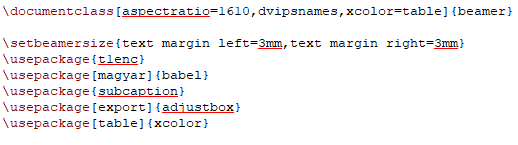
\includegraphics[scale=0.8]{img/tablesetup.png}
			 \onslide<2->\caption{Felállítás}
	\end{figure}
\end{frame}

\begin{frame}[fragile]{Táblázat színezés}
\begin{center}
\LaTeX-ben való alkalmazás
\noindent
{\color{Dandelion} \rule{\linewidth}{1mm}}
\end{center}
	\begin{figure}[H]
		\onslide<2->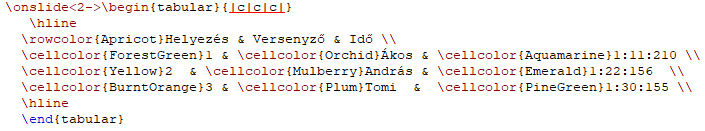
\includegraphics[scale=0.8]{img/tablealkalmazas.png}
			 
	\end{figure}
\end{frame}

\begin{frame}[fragile]{Vége}
\begin{center}
\Huge Köszönjük a figyelmet!
\end{center}
\end{frame}

\end{document}